\section{Theoretical Analysis}
\label{sec:analysis}

In this section, the circuit shown in \textbf{Figure~\ref{fig:diagram_t2}} is analysed
theoretically.
\begin{figure}[H] \centering
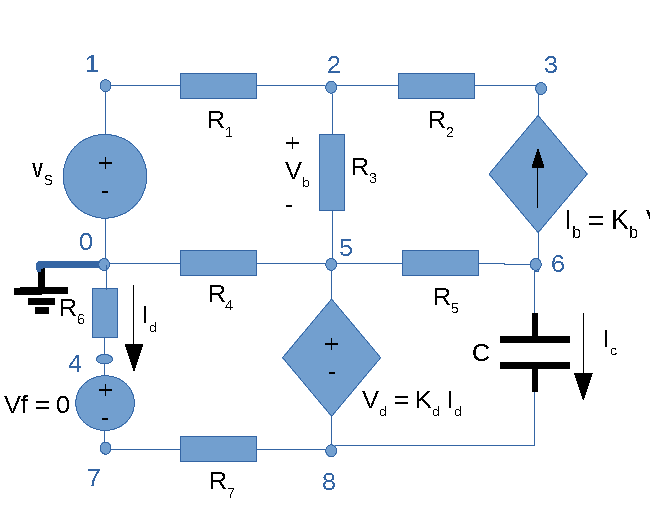
\includegraphics[width=0.6\linewidth]{diagram_t2.pdf}
\caption{Diagram of the circuit considered for the computations and simulations}
\label{fig:diagram_t2}
\end{figure}

%point 1
\subsection{Analysis for $t<0$} 
The nodal method is aplied to the circuit in order to determine the voltage in all nodes and the current on all branches . The nodal method aplies KVL and for $t<0$ no current passes through the capacitor, and therefore this component behaves like an open circuit.
%In \textbf{Table~\ref{tab:theoretical}} the values for the branch currents and the node voltages obtained from the Octave script for both methods are presented. Here, the node voltages in the mesh method were computed from the respective currents, which were determined as described in the previous subsection.

\begin {equation}
	V_0 = 0
	\label{eq:n1}
\end{equation}
\begin {equation}
	V_4 = V_7
	\label{eq:n2}
\end{equation}
\begin {equation}
	V_5 - V_8 = K_d \frac{V_0 - V_4}{R_6}
	\label{eq:n3}
\end{equation}
\begin {equation}
	V_1 - V_0 = V_s
	\label{eq:n4}
\end{equation}
\begin {equation}
	\frac{V_2-V_1}{R_1} + \frac{V_2 - V_5}{R_3} + \frac{V_2 - V_3}{R_2} = 0
	\label{eq:n5}
\end{equation}
\begin {equation}
	\frac{V_3-V_2}{R_2} - K_b(V_2-V_5)  = 0
	\label{eq:n6}
\end{equation}
\begin {equation}
	\frac{V_5-V_2}{R_3} + \frac{V_5-V_0}{R_4} + \frac{V_5-V_6}{R_5} + \frac{V_8-V_7}{R_7}= 0
	\label{eq:n7}
\end{equation}
\begin {equation}
	K_b(V_2-V_5) + \frac{V_6-V_5}{R_5}   = 0
	\label{eq:n8}
\end{equation}
\begin {equation}
	\frac{V_4-V_0}{R_6} + \frac{V_7 - V_8}{R_7} = 0
	\label{eq:n9}
\end{equation}



\begin{table}[H]
\parbox{.45\linewidth}{
  \centering 
  \begin{tabular}{|l|r|}
    \hline    
    {\bf Name} & {\bf Node method}\\ \hline
    V0 & 0\\ \hline
V1 &  5.054818641360000\\ \hline
V2 &  4.793704691824189\\ \hline
V3 &  4.258197784082119\\ \hline
V4 & -1.934225550007436\\ \hline
V5 &  4.831047093349573\\ \hline
V6 &  5.668298372306746\\ \hline
V7 & -1.934225550007436\\ \hline
V8 & -2.905231322705667\\ \hline
Ir1 &   -2.536487650531725e-01\\ \hline
Ir2 &   -2.658975828505401e-01\\ \hline
Ir3 &    1.224881779736725e-02\\ \hline
Ir4 &  1.205310280142027\\ \hline
Ir5 &    2.658975828505403e-01\\ \hline
Ir6 &   -9.516615150888543e-01\\ \hline
Ir7 &   -9.516615150888547e-01\\ \hline
Gbn &    2.658975828505403e-01\\ \hline

  \end{tabular}
  \caption{A variable that starts with "@ " is of type {\em current}
    and expressed in milliampere (mA); all the other variables that start with a "V" are of the type {\it voltage} and expressed in
    Volt (V).}
  \label{tab:theoretical}
  
 }
 \hfill
 \parbox{.45\linewidth}{
 \centering
  \begin{tabular}{|l|r|}
    \hline    
    {\bf Name} & {\bf Simulation} \\ \hline
    @c[i] & 0.000000e+00\\ \hline
@gb[i] & -2.91567e-04\\ \hline
@r1[i] & 2.780494e-04\\ \hline
@r2[i] & 2.915672e-04\\ \hline
@r3[i] & -1.35178e-05\\ \hline
@r4[i] & -1.22689e-03\\ \hline
@r5[i] & -2.91567e-04\\ \hline
@r6[i] & 9.488377e-04\\ \hline
@r7[i] & 9.488377e-04\\ \hline
v(1) & 5.243596e+00\\ \hline
v(2) & 4.952739e+00\\ \hline
v(3) & 4.367468e+00\\ \hline
v(4) & -1.96340e+00\\ \hline
v(5) & 4.994112e+00\\ \hline
v(6) & 5.904536e+00\\ \hline
v(7) & -1.96340e+00\\ \hline
v(8) & -2.92677e+00\\ \hline

  \end{tabular}
  \caption{Step 1: Operating point for $t<0$. A variable preceded by @ is of type {\em current}
    and expressed in miliAmpere; other variables are of type {\it voltage} and expressed in
    Volt.}
  \label{tab:op}
 
 }
\end{table}


%point 2
\subsection{Equivalent resistor as seen from the capacitor terminals}

To compute the equivalent resistance as seen by C the independent source $V_c$ needs to be switched off. We do this by replacing it with a short circuit ($V_s=0$). In addition, due to the presence of dependent sources, we also needed to replace the capacitor with a voltage source $V_x=V_6-V_8$. We use the $V_6$ and $V_8$ from the previous section beacause the voltage drop at the terminals of the capacitor needs to be a continuous function (there can not be an energy discontinuity in the capacitor). With this in mind, a nodal analysis is performed in order to determine the current $I_x$ that is supplied by $V_x$. With these values we can determine $R_{eq}$ ($R_{eq}=V_x/I_x$). All these procedures were required in order to determine the time constant $\tau$ ($\tau=R_{eq}*C$). The time constant is crucial to determine the natural and forced solutions for $V_6$, which will be done in the next subsections. The equations considered for these calculations were \ref{eq:n1}, \ref{eq:n2}, \ref{eq:n3}, \ref{eq:n4}, \ref{eq:n5}, \ref{eq:n6} and the following:

%In \textbf{Table~\ref{tab:theoretical}} the values for the branch currents and the node voltages obtained from the Octave script for both methods are presented. Here, the node voltages in the mesh method were computed from the respective currents, which were determined as described in the previous subsection.

\begin {equation}
	\frac{V_1-V_2}{R_1} + \frac{V_0-V_4}{R_6} + \frac{V_0-V_5}{R_4} = 0
	\label{eq:eq7}
\end{equation}
\begin {equation}
	K_b(V_2-V_5) + \frac{V_6-V_5}{R_5} + I_x  = 0
	\label{eq:eq8}
\end{equation}
\begin {equation}
	\frac{V_4-V_0}{R_6} + \frac{V_7 - V_8}{R_7} = 0
	\label{eq:eq9}
\end{equation}
\begin {equation}
	V_x = V_6 - V_8
	\label{eq:eq10}
\end{equation}


\begin{table}[H]
\parbox{.40\linewidth}{
  \centering
  \begin{tabular}{|l|r|}
    \hline    
    {\bf Name} & {\bf Theoretical values }\\ \hline
    @Gb & 0.00000000000\\ \hline
@r1 & 0\\ \hline
@r2 & 0\\ \hline
@r3 & 0\\ \hline
@r4 & 0\\ \hline
@r5 &   -2.828260531660058e-03\\ \hline
@r6 & 0\\ \hline
@r7 & 0\\ \hline
v(1) & 0.00000000000\\ \hline
v(2) & 0.00000000000\\ \hline
v(3) & 0.00000000000\\ \hline
v(4) & 0.00000000000\\ \hline
v(5) & 0.00000000000\\ \hline
v(6) & 8.83130397945\\ \hline
v(7) & 0.00000000000\\ \hline
v(8) & 0.00000000000\\ \hline
Ix & -0.00282826053\\ \hline
Vx & 8.83130397945\\ \hline
$Req_{}$ & -3.122521e+03\\ \hline
$\tau$ & -3.181599e-03\\ \hline
  \end{tabular}
  \caption{A variable that starts with a "V" is of type {\it voltage} and expressed in
    Volt (V). The variable $R_{eq}$ is expressed in Ohm and the variable $\tau$ is expressed in seconds }
  \label{tab:equivalent resistor}
}
 \hfill
 \parbox{.35\linewidth}{
  \centering
  \begin{tabular}{|l|r|}
    \hline    
    {\bf Name} & {\bf Simulation values } \\ \hline
    @gb[i] & 4.151983e-18\\ \hline
@r1[i] & -3.95949e-18\\ \hline
@r2[i] & -4.15198e-18\\ \hline
@r3[i] & 1.924970e-19\\ \hline
@r4[i] & -8.72784e-19\\ \hline
@r5[i] & -2.82826e-03\\ \hline
@r6[i] & 4.336809e-19\\ \hline
@r7[i] & -8.83871e-19\\ \hline
v(1) & 0.000000e+00\\ \hline
v(2) & 4.141871e-15\\ \hline
v(3) & 1.247625e-14\\ \hline
v(4) & -8.97403e-16\\ \hline
v(5) & 3.552714e-15\\ \hline
v(6) & 8.831302e+00\\ \hline
v(7) & -8.97403e-16\\ \hline
v(8) & 0.000000e+00\\ \hline
Ix & -2.82826e-03\\ \hline
Vx & 8.831302e+00\\ \hline
Req & -3.12252e+03\\ \hline

  \end{tabular}
  \caption{Step 2: Operating point for {\it $v_s(0)=0$}. A variable preceded by @ is of type {\em current}
    and expressed in miliAmpere; variables are of type {\it voltage} and expressed in
    Volt. The equivalent resistance is in Ohms}
  \label{tab:opeq}
  }
\end{table}



\pagebreak
%point 3
\subsection{Natural solution for $V_6$}

The natural solution depends on the initial charge (voltage), on $R_{eq}$ and C and it is computed by removing all independent sources and applying KVL. In Octave, to compute the Natural solution the general formula derived in the theoretical classes was used: $V_{6n}(t)=Ae^{\frac{-t}{\tau}}$. In this formula $\tau$ is the time constant determined in the previous section and  A is a constant that can be determined through the boundary conditions (when $t=0$, $A=V_x$).

\begin{figure}[H] \centering
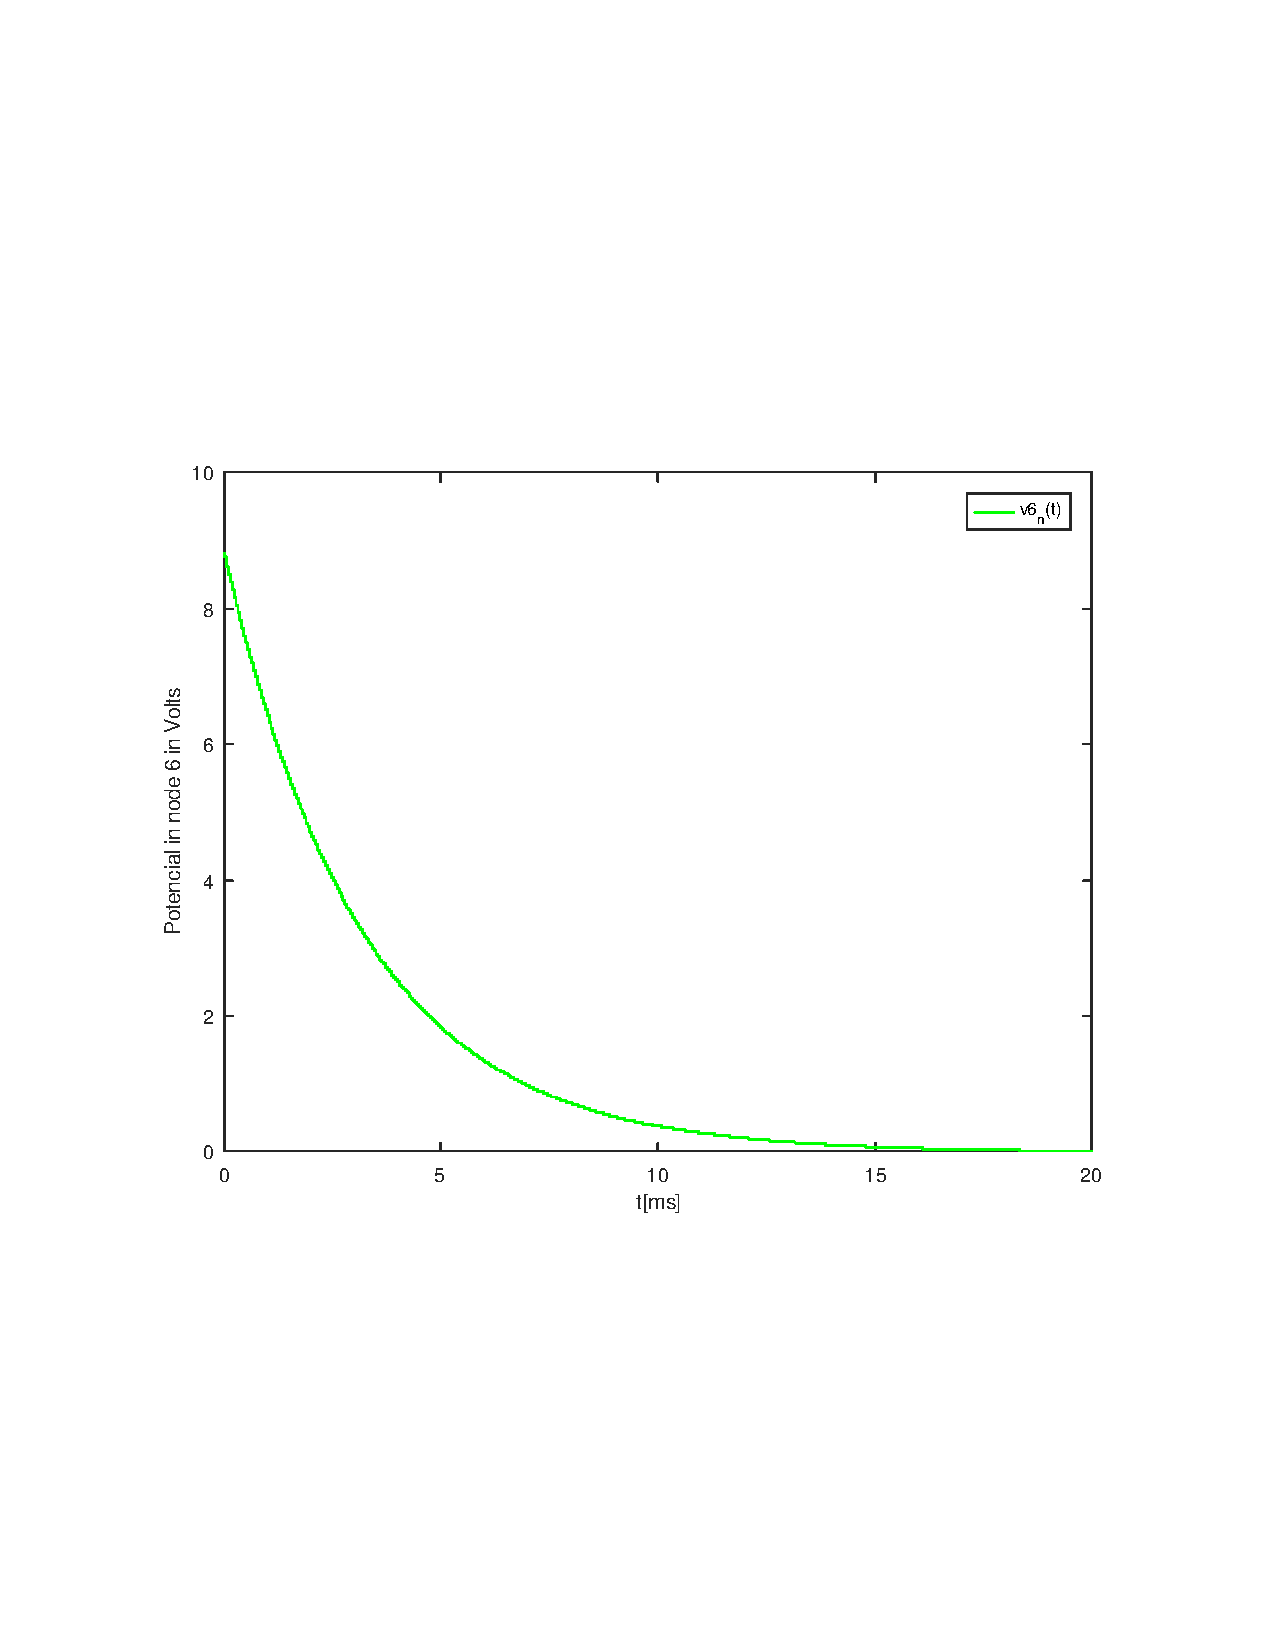
\includegraphics[width=0.9\linewidth]{natural_tab.pdf}
\caption{Natural response of $V_6$ as a function os time in the interval from [0,20] ms}
\label{fig:natural}
\end{figure} 


\pagebreak
%point 4
\subsection{Forced solution for $V_6$ with $f=1000Hz$}

In this section the forced solution $V_{6f}$ is determined for the same time interval and for a frequency of 1KHz. To do this a nodal analysis was used, but insted of resistances and capacitances, impedances were used. It was also  considered that the magnitude of the phasor representing the voltage sorce $\tilde{V}_s$ was 1 ($V_s=1$), a result of expression \ref{eq:i1}. By taking all these steps the phasor voltages in all nodes were determined in accordance to the following equations:

\begin {equation}
	Z = \frac{1}{w C j}
	\label{eq:Z}
\end{equation}

\begin {equation}
	\tilde{V}_s = -j
	\label{eq:vs}
\end{equation}

\begin {equation}
	\tilde{V}_0 = 0
	\label{eq:p1}
\end{equation}
\begin {equation}
	\tilde{V}_4 = \tilde{V}_7
	\label{eq:p2}
\end{equation}
\begin {equation}
	\tilde{V}_5 - \tilde{V}_8 = K_d \frac{\tilde{V}_0 - \tilde{V}_4}{R_6}
	\label{eq:p3}
\end{equation}
\begin {equation}
	\tilde{V}_1 - \tilde{V}_0 = \tilde{V}_s
	\label{eq:p4}
\end{equation}
\begin {equation}
	\frac{\tilde{V}_2-\tilde{V}_1}{R_1} + \frac{\tilde{V}_2 - \tilde{V}_5}{R_3} + \frac{\tilde{V}_2 - \tilde{V}_3}{R_2} = 0
	\label{eq:p5}
\end{equation}
\begin {equation}
	\frac{\tilde{V}_3-\tilde{V}_2}{R_2} - K_b(\tilde{V}_2-\tilde{V}_5)  = 0
	\label{eq:p6}
\end{equation}
\begin {equation}
	\frac{\tilde{V}_1-\tilde{V}_2}{R_1} + \frac{\tilde{V}_0-\tilde{V}_4}{R_6} + \frac{\tilde{V}_0-\tilde{V}_5}{R_4} = 0
	\label{eq:p7}
\end{equation}
\begin {equation}
	K_b(\tilde{V}_2-\tilde{V}_5) + \frac{\tilde{V}_6-\tilde{V}_5}{R_5} + \frac{\tilde{V}_6-\tilde{V}_8}{Z}  = 0
	\label{eq:p8}
\end{equation}
\begin {equation}
	\frac{\tilde{V}_4-\tilde{V}_0}{R_6} + \frac{\tilde{V}_7 - \tilde{V}_8}{R_7} = 0
	\label{eq:p9}
\end{equation}
\begin {equation}
	\tilde{V}_x = \tilde{V}_6 - \tilde{V}_8
	\label{eq:p10}
\end{equation}


The complex amplitudes of the phasors are presented in  \textbf{Table ~\ref{tab:equivalent resistor}}
\begin{table}[H]
  \centering
  \begin{tabular}{|l|r|}
    \hline    
    {\bf Name} & {\bf Complex amplitude voltage}\\ \hline
    V0 & 0\\ \hline
V1 &  1\\ \hline
V2 &    9.445310207903378e-01\\ \hline
V3 &    8.329148493139050e-01\\ \hline
V4 &    3.744381306846604e-01\\ \hline
V5 &    9.524211706387480e-01\\ \hline
V6 &    5.602948262043124e-01\\ \hline
V7 &    3.744381306846604e-01\\ \hline
V8 &    5.581602943867834e-01\\ \hline

  \end{tabular}
  \caption{Complex amplitudes in all nodes in Volts}
  \label{tab:equivalent resistor}
\end{table}
\vspace{10cm}

\pagebreak
%point 5
\subsection{Final total solution $v_6(t)$}
In this section the final total solution $V_6$ for a frequency of 1KHz is determined by superimposing the natural and forced solutions determined in previous sections ($V_6$=$V_{n6}$+$V_{6f}$) In \textbf{Figure: ~\ref{fig:theo5}} the voltage of the independent source $V_{s}$ and the voltage of $V_{6}$ were plotted for the time interval of [-5,20] ms. 
\begin{figure}[h!] \centering
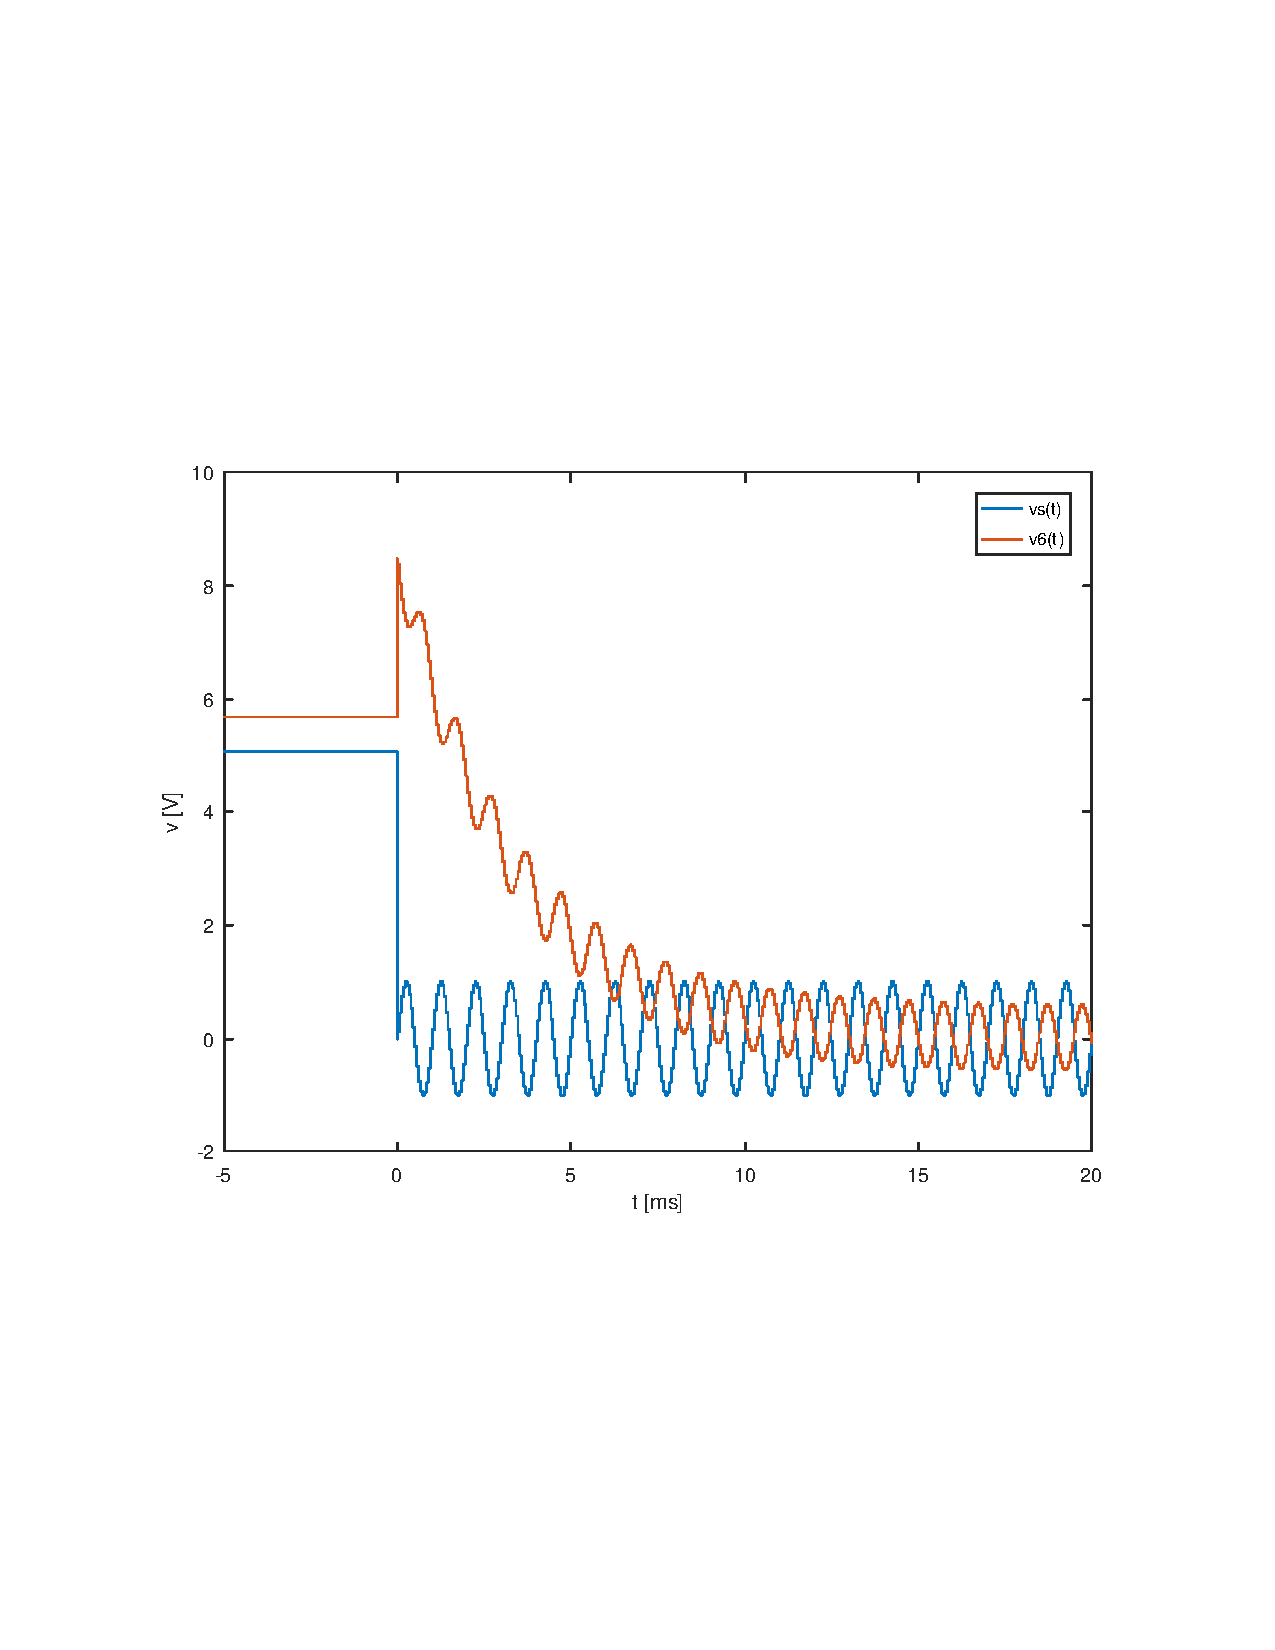
\includegraphics[width=0.9\linewidth]{theo5_tab.pdf}
\caption{Voltage of $V_{6}(t)$ and $V_{s}(t)$ as functions of time from [-5,20] ms}
\label{fig:theo5}
\end{figure}
\vspace{15cm}


\pagebreak
\subsection{Frequency responses $v_c(f)$, $v_s(f)$ and $v_6(f)$ for frequency range 0.1 Hz to 1 MHz}
\label{ref}
For this section, we considered $v_s( t)  = sin( 2 \pi f t )$. As we can see, the magnitude and the phase do not depend on the frequency $f$. Therefore, we are to expect these values to remain constant for both these variables in the figures \ref{fig:freq_resp} and \ref{fig:angle_resp}.\par 
This circuit can serve the purpouse of a low-pass filter.
In other words, when the frequencies are low, there is plenty of time for the capacitor 
to charge up to practically the same voltage as the input, which means
it will act aproximately as an open circuit, thus allowing a considerable potential drop 
from nodes 6 to 8.This means that for low frequencies the voltage in the capacitor
is in phase with the voltage source. However when the frequencies are high, 
the capacitor only has a small time to charge up before the input changes direction, which 
means it will act aproximately as a short-circuit. Therefore, there will be close to none 
potential drop between nodes 6 and 8 and the capacitor and source will start to fall 
out of phase, for frequencies greater that the cutoff frequecy ($f_c$). 
This frequency can be calculated with the following formula. $f_c = \frac{1}{2.\pi.\tau}$.  
For the values provided this cutoff frequency is around 50Hz. This explains the steep drop 
in potential difference that we can see in the graph around the first and second decades.
The phase difference between the capacitor voltage and the voltage source also begins to 
show at around this frequency as can be seen in \textbf{Figure: ~\ref{fig:angle_resp}}.\par
Simplifying the circuit to a voltage source, capacitor and equivalent resistor yields the following equations, which help understand the phase and magnitude declination with the increase in frequency: 

\begin{equation}
  V_c = \frac{V_s}{\sqrt{1 + (R_{eq}.C.2\pi.f)^2}}
  \label{eq:freqresp1}
\end{equation}

\begin{equation}
  \phi_{V_c} = -\frac{\pi}{2} + arctan(R_{eq}.C.2\pi.f)
  \label{eq:freqresp2}
\end{equation}

\begin{figure}[H] \centering
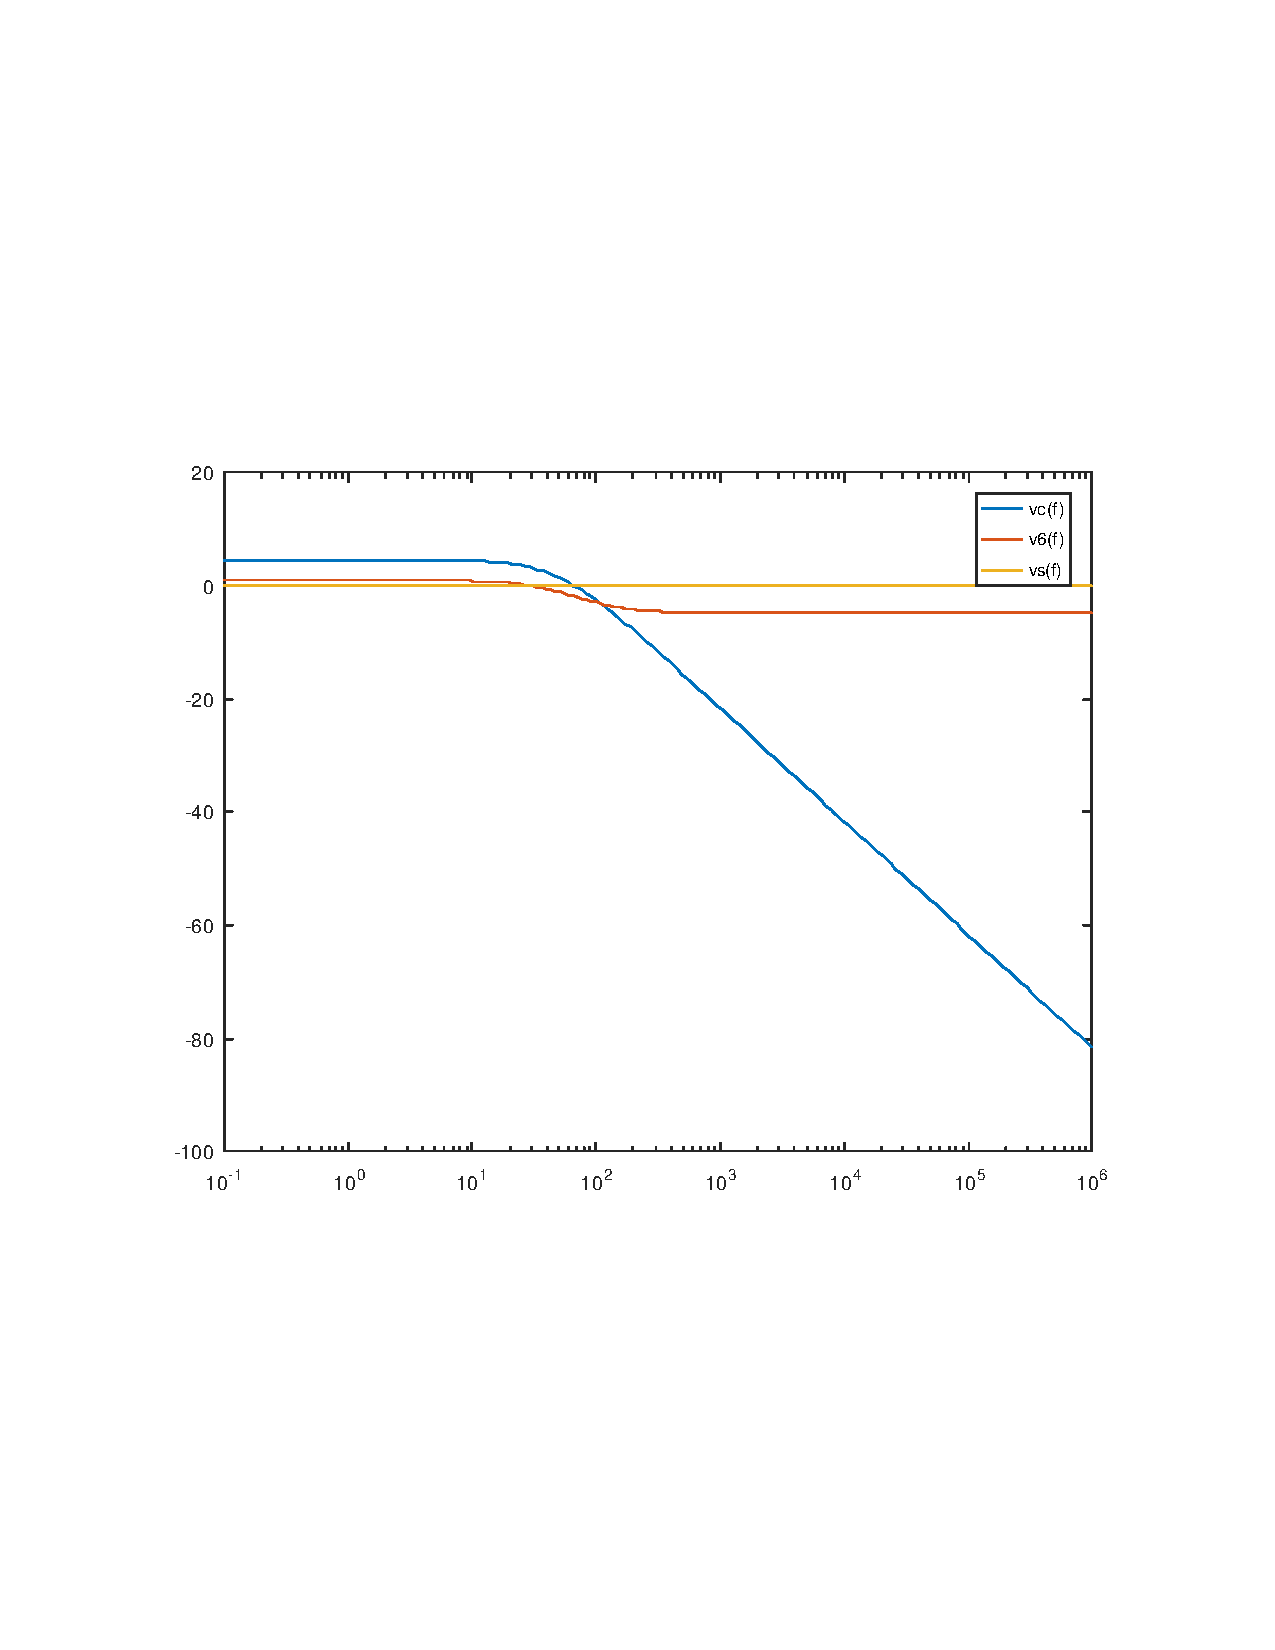
\includegraphics[width=0.9\linewidth]{freq_resp_tab.pdf}
\caption{Graph for amplitude frequency response, in dB, of $V_c$, $V_6$ and $V_s$ for frequencies ranging from 0.1Hz to 1MHz (logarithmic scale).}
\label{fig:freq_resp}
\end{figure}



\begin{figure}[H] \centering
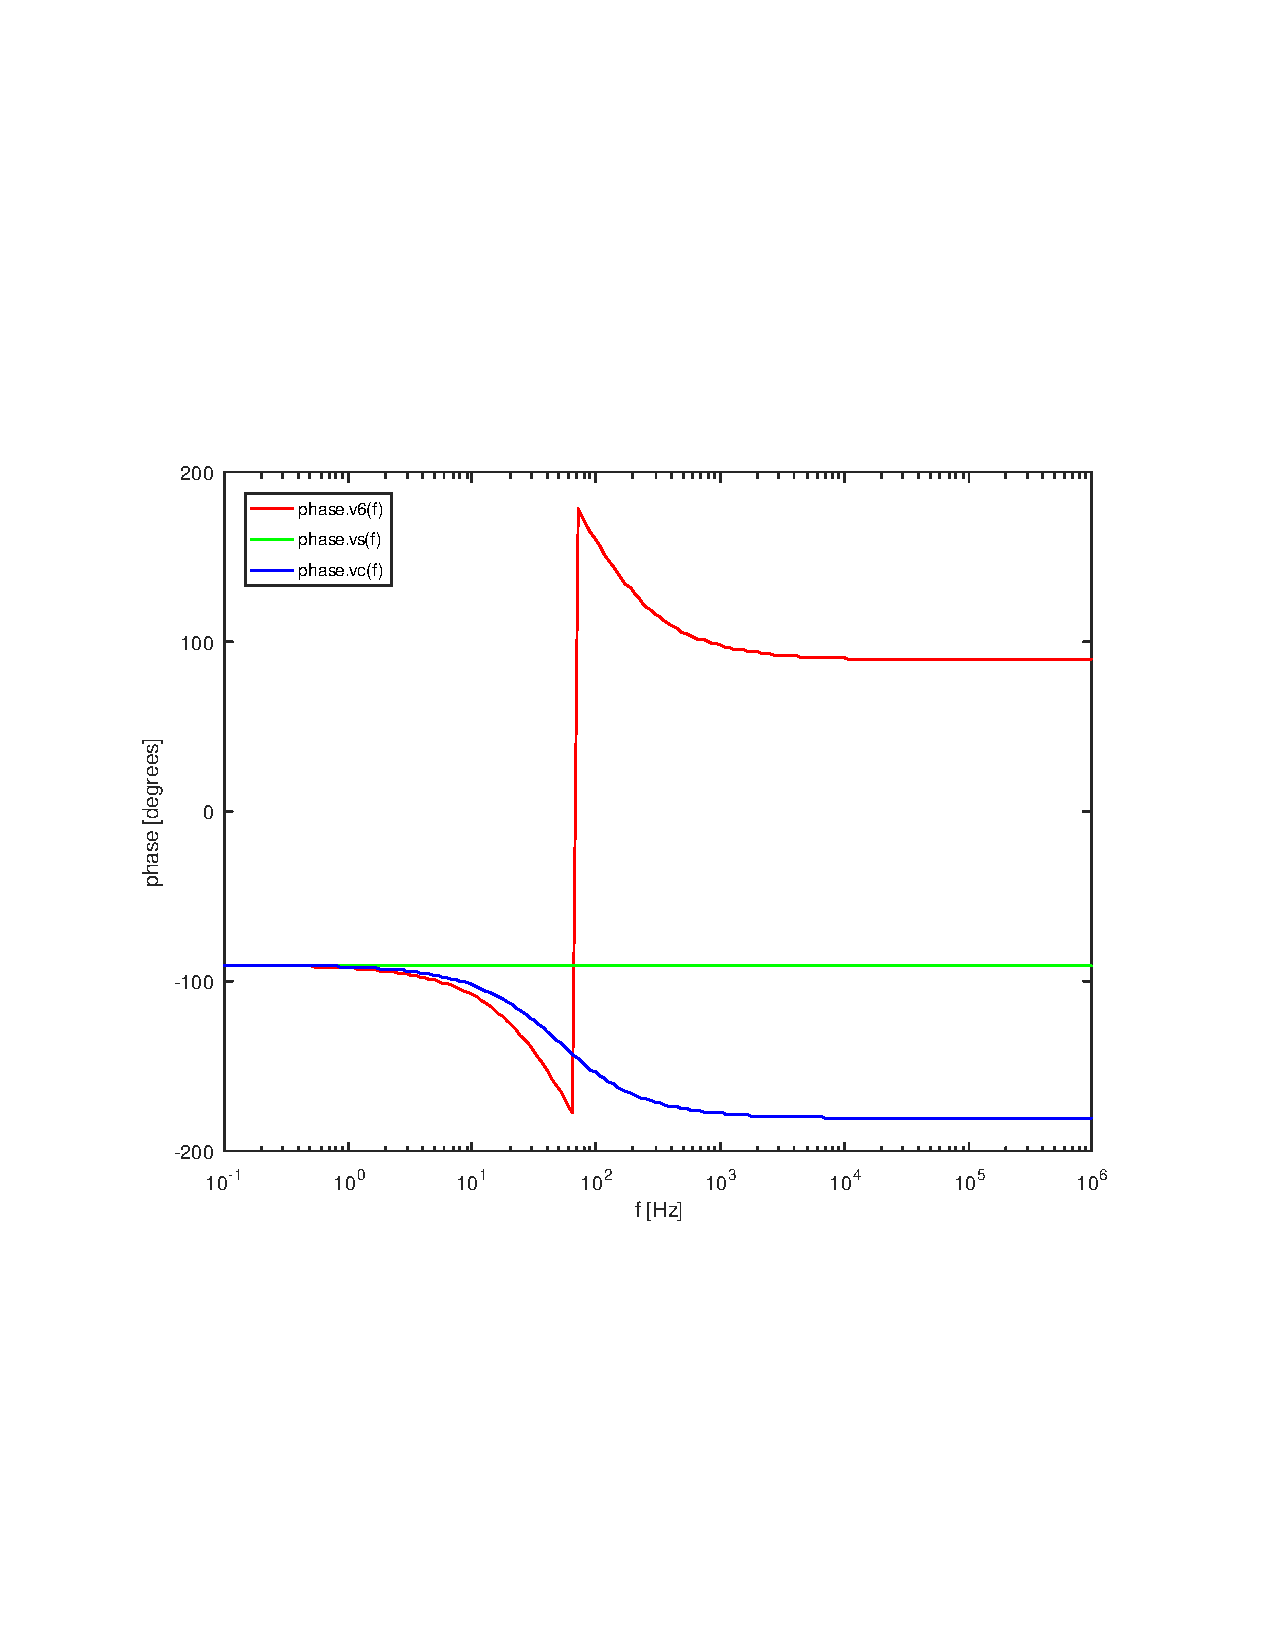
\includegraphics[width=0.9\linewidth]{angle_tab.pdf}
\caption{Graph for the phase response, in degrees of $V_c$, $V_6$ and $V_s$ for frequencies ranging from 0.1Hz to 1MHz, displayed in a logarithmic scale. Note that the apparent peak discontinuity in the phase of $V_6$ is only due to the domain of the arctan function that gives the phase (angle of the phasor), and so the phase is in fact continuous.}
\label{fig:angle_resp}
\end{figure}

\pagebreak


